\documentclass[handout, xcolor=dvipsnames,aspectratio=169]{beamer}
\usecolortheme[dark,accent=cyan]{solarized}
\usepackage[utf8]{inputenc}
\usepackage{multicol}
\usepackage{url}
\usepackage{hyperref}
\usepackage{subfig}
\title{Cryptography}
\author{Gaspare Ferraro\\ ferraro@gaspa.re}
\subtitle{Hands-on session}


\begin{document}

\begin{frame}[plain]
  \maketitle
  \begin{columns}
    \column{0.5\textwidth}
    \center {
      \includegraphics[width=0.3\textwidth]{style/qrcode.png}\\
      \href{https://zenhack.it}{visit us!}
    }
    \column{0.5\textwidth}
    \center{
      \includegraphics[width=0.3\textwidth]{style/gaspare.jpg}\\
      \href{https://t.me/GaspareG}{@GaspareG}
    }

  \end{columns}
\end{frame}

%%%%%%%%%%%%%%%%%%%%%%%%%%%%%%%%%%%%%%%%%%%%%%%%%%%%%%%%%%%%%%%%%%%%%%%%%%%%%%%
%%%%%%%%%%%%%%%%%%%%%%%%%%%%%%%%%%%%%%%%%%%%%%%%%%%%%%%%%%%%%%%%%%%%%%%%%%%%%%%

\part{Introduction}

\begin{frame}
  \partpage
  \centering
\end{frame}

\begin{frame}{Disclaimer 1: What crypto \textbf{is not}}

  \center {

    Crypto \textbf{is not} Cryptocurrency

    \medskip

    \pause

    \includegraphics[width=0.3\textwidth]{img/crypto}

    \medskip

    \url{https://www.cryptoisnotcryptocurrency.com/}

    \medskip

    \includegraphics[width=0.3\textwidth]{img/blockchain}

    \pause


    \medskip

    crittografia = kryptós + graphía (let. \textit{scrittura nascosta})
  }

\end{frame}


\begin{frame}{Disclaimer 2: What crypto \textbf{is}}

  \center {

    Large use of {\color{red} \textit{math}}!

    \medskip

    \pause

    \includegraphics[width=0.5\textwidth]{img/meme}

    \medskip

    \pause

    Back to the past...
  }

\end{frame}

\begin{frame}{"Ancient" cryptography}

  \pause

  \begin{figure}%
    \centering
    \subfloat[Caesar cipher]{{
          \centering\includegraphics[width=5cm]{img/cesaer.png} }}%
    \pause
    \qquad
    \subfloat[Scytala]{{
          \centering\includegraphics[width=5cm]{img/scitala.png} }}%
  \end{figure}

\end{frame}

\begin{frame}{"Mechanical" cryptography}

  \centering

  \includegraphics[width=0.6\textwidth]{img/enigma}

  Enigma: electro-mechanical machine to encrypt and decrypt messages\\
  used by the Nazis during World War II.

\end{frame}


\begin{frame}{Cryptography today}
  \center {
    The needs, as well as the resources available, have evolved

    and today we can divide cryptography into:

    \pause

    \medskip
    \includegraphics[width=0.6\textwidth]{crypto-section.pdf}
  }
\end{frame}

\begin{frame}{Symmetric and Asymmetric encryption}

  \pause

  \begin{figure}%
    \centering
    \subfloat[Padlock with code]{{
          \centering\includegraphics[width=5cm]{img/symmetric.jpg} }}%
    \pause
    \qquad
    \subfloat[Padlock with key]{{
          \centering\includegraphics[width=5cm]{img/asymmetric.jpg} }}%
  \end{figure}


\end{frame}

%%%%%%%%%%%%%%%%%%%%%%%%%%%%%%%%%%%%%%%%%%%%%%%%%%%%%%%%%%%%%%%%%%%%%%%%%%%%%%%
%%%%%%%%%%%%%%%%%%%%%%%%%%%%%%%%%%%%%%%%%%%%%%%%%%%%%%%%%%%%%%%%%%%%%%%%%%%%%%%

\part{Symmetric cryptography}

\begin{frame}
  \partpage
  \centering
\end{frame}

\begin{frame}{Symmetric cryptography}

  \pause

  Symmetric ciphers are those where messages $ m $ are encrypted and decrypted using the same key $ k $, which must be known only and exclusively to both parties.

  \medskip

  \pause
  $\mathcal{C}(m, k) = c$ (Encryption function)

  $\mathcal{D}(c, k) = m$ (Decryption function)

  \medskip

  Obviously it must hold true:

  $\mathcal{D}(\mathcal{C}(m, k), k) = m$ (the original message is not altered during the exchange).

  \medskip
  \pause

  For example in Caesar Cipher:

  $\mathcal{C}(m, k) = $ Shift forward each character of $k$ position.

  $\mathcal{D}(c, k) = $ Shift backward each character of $k$ position.

\end{frame}

%%%%%%%%%%%%%%%%%%%%%%%%%%%%%%%%%%%%%%%%%%%%%%%%%%%%%%%%%%%%%%%%%%%%%%%%%%%%%%%
\begin{frame}{ROT\{13, 47\}}

  \centering

  \medskip

  ROT13: Caesar cipher with $ K = 13 $ on alphabet A-Z.

  ROT47: Caesar cipher with $ K = 47 $ on ASCII dictionaries (33 - 126).

  \medskip

  \includegraphics[width=8cm]{img/ROT13.png}

  \medskip

  Why $K = 13$ (or $K = 47$)?
  Because \textcolor{red}{Encrypt = Decrypt}

\end{frame}

\begin{frame}{Classical Ciphers}

  \textbf{Substitution Ciphers}

  \phantom{pad}- Mono-alphabetic Ciphers: \textcolor{red}{$C_{new} = P[C_{old}]$} (Where $P$ is an alphabet permutation)

  \smallskip

  \phantom{pad}(ROT-K is a mono-alphabetic cipher where $ P $ is a cyclic rotation)

  \smallskip

  \phantom{pad}- Poly-alphabetic ciphers: characters are replaced using \textcolor{red}{multiple dictionaries}

  \smallskip

  \textbf{Transposition Ciphers}

  \phantom{pad}Ciphers where the \textcolor{red}{positions}, (of one character or multiple characters) of the message, are \textcolor{red}{transposed} according to a specific system.

  \smallskip

  E.g. We want to cipher the message \textit{WE ARE DISCOVERED. FLEE AT ONCE}

  using the \textbf{route cipher}:

  Grid:

  \centerline{\texttt{W R I O R F E O E}}
  \centerline{\texttt{E E S V E L A N J}}
  \centerline{\texttt{A D C E D E T C X}}

  Message: \textit{EJXCTEDECDAEWRIORFEONALEVSE}

\end{frame}

%%%%%%%%%%%%%%%%%%%%%%%%%%%%%%%%%%%%%%%%%%%%%%%%%%%%%%%%%%%%%%%%%%%%%%%%%%%%%%%
\begin{frame}{dcode.fr}

  \centering

  \href{https://www.dcode.fr/tools-list}{https://www.dcode.fr/tools-list}

  \medskip

  \includegraphics[width=8cm]{img/dcode.png}

  \medskip

  \textcolor{red}{Almost} all possible classical ciphers (and not), ancient and modern, encoder/decoder, ...

\end{frame}
%%%%%%%%%%%%%%%%%%%%%%%%%%%%%%%%%%%%%%%%%%%%%%%%%%%%%%%%%%%%%%%%%%%%%%%%%%%%%%%
\begin{frame}{CyberChef}

  \centering

  \href{https://gchq.github.io/CyberChef/}{https://gchq.github.io/CyberChef/}

  \medskip

  \includegraphics[width=9cm]{img/cyberchef.jpg}

  \medskip

  CyberChef - The Cyber Swiss Army Knife

\end{frame}
%%%%%%%%%%%%%%%%%%%%%%%%%%%%%%%%%%%%%%%%%%%%%%%%%%%%%%%%%%%%%%%%%%%%%%%%%%%%%%%


\begin{frame}{XOR cipher}

  Consider the XOR operation $\oplus$ (exclusive or), it holds the properties:

  \begin{itemize}
    \item $0 \oplus 0 = 1 \oplus 1 = 0$
    \item $0 \oplus 1 = 0 \oplus 1 = 1$
    \item $x \oplus y \oplus y = x$
  \end{itemize}

  \medskip
  \pause

  We define the XOR cipher as:

  $\mathcal{C}(m, k) = m \oplus k$

  $\mathcal{D}(c, k) = c \oplus k$

  \medskip

  \pause

  Problem: the key $k$ could be shorter than the message $m$.

  Solution: Repeat the key: $k^{'} = k \cdot k \cdot \ldots \cdot k$ until it reaches (or exceeds) the length of $m$.

  \medskip
  \pause

  Example:

  \texttt{m = 01100011 01101001 01100001 01101111} (ciao in ASCII).\\
  \texttt{k = 01111000 01111000 01111000 01111000} (x in ascii 4 times)\\
  \texttt{c = 00011011 00010001 00011001 00010111} (non printable, \texttt{GxEZFw==} in b64)


\end{frame}

\begin{frame}{One-time Pad}

  \pause

  The problem with the XOR cipher is that encrypting using the same key repeatedly can leak \textit{statistical} information about the original message.
  \medskip

  \pause
  We are therefore talking about Vernam's cipher (or one-time pad) when the length of the key is equal to that of the message, this cipher is called \textit{perfect} because it holds:
  \medskip

  $P(M = m | C = c) = P(M = m)$

  \medskip

  That is the probability that $ M $ is a certain message knowing that the cipher is $ C $ is equal to the probability that $ M $ is a certain message not knowing the cipher (all messages are equally likely, the encrypted message does not provide us with information on key used).

  \medskip

  \pause

  Beatiful, but:

  \begin{itemize}
    \item The key must be exchanged using a secure method (exchange \textit{by hand}).
    \item The key must be randomly generated and not reused (otherwise a many-time pad attack is possible).
  \end{itemize}

\end{frame}


\begin{frame}{Statistical cryptanalysis}

  \pause

  Often the vulnerability is not in the algorithm but in its application ...

  \pause

  \medskip

  \begin{itemize}
    \item The key is too short for the message
    \item The key is repeated several times to encrypt different messages
    \item Messages use a poorly distributed dictionary.
    \item We know the message format (ex: \texttt{flag\{$\ldots$\}})
  \end{itemize}

  \medskip

  \pause

  In particular, we speak of statistical cryptanalysis when we force the cipher not from an algorithmic point of view but from a statistical one.

  \pause

  For example in Italian the $33\%$ of the letters used is one of the vowels \texttt{a, e, i} while only with probability of $0.5\% $ it will be a \texttt{z} or a \texttt{q}.

\end{frame}

\begin{frame}{Statistical cryptanalysis}

  \centering

  Useful tool for statistical analysis of encrypted messages:

  \includegraphics[width=5.5cm]{img/xortool}

  \pause

  Knowing the initial part you can see some clear words:

  \centering\includegraphics[width=4cm]{img/xor1}

  Trying to reconstruct the final flag:

  \centering\includegraphics[width=4cm]{img/xor2}

\end{frame}

\begin{frame}{Many-Time Pad Interactive}

  \url{https://github.com/CameronLonsdale/MTP}

  \smallskip

  \centering\includegraphics[width=8cm]{img/MTP}

  \smallskip

  \textit{"MTP Interactive uses automated cryptanalysis to present a partial decryption which can be solved interactively."}


\end{frame}

\begin{frame}{Shannon's principles}

  \pause
  How to evaluate if a cipher is strong enough? (Where robustness means its possibility of being successfully attacked).
  \medskip
  \pause
  Shannon defines two key concepts:

  \begin{itemize}
    \item Confusion: the key must be well distributed in the cipher (every bit of the cipher should depend on every bit of the key).
    \item Diffusion: the message must be well distributed in the cipher (every bit of the cipher should depend on every bit of the message).
  \end{itemize}

  \medskip
  \pause

  In the case of the Caesar cipher we have no type of diffusion and low confusion (why?).

\end{frame}


\begin{frame}{DES \& AES}

  Data Encryption Standard (DES) and Advanced Encryption Standard (AES) are based on the concept of the \textit{S-Box} (Substitution box).

  \pause

  \medskip

  \centering\includegraphics[width=5cm]{img/des}

  \medskip

  Confusion and diffusion are implemented by performing a (large) number of invertible operations.

\end{frame}

\begin{frame}{DES, 2DES, 3DES}

  The DES algorithm, released in 1975, uses a 56-bit \ textit {only} key.

  It remained standard until 1999, when a group of researchers managed to crack an encryption key in just 22 hours.

  With today's computing power a few hours would be enough.

  \begin{columns}
    \begin{column}{0.5\textwidth}
      \medskip

      Before introducing AES, a more \textit{robust} (and immediate) alternative to the now violated DES algorithm was to repeat DES 3 times (the 3DES algorithm: encryption-decryption-encryption).

      \medskip

      Why 3DES and not 2DES?

      \medskip

      Using 2 56-bit keys I would expect the same security as a 112-bit key, but that's not the case ...
    
    \end{column}
    \begin{column}{0.5\textwidth}  %%<--- here
      \begin{center}
        \includegraphics[width=0.7\textwidth]{img/2des}
      \end{center}
    \end{column}
  \end{columns}


\end{frame}


\begin{frame}{Meet-In-The-Middle Attack}

  \small

  \textsc{C = 2DES$_{enc}$(M, k$_1$, k$_2$) = DES$_{enc}$(DES$_{enc}$(M, k$_2$), k$_1$)}

  \medskip

  \textsc{C$_1$ = DES$_{enc}$(M, k$_1$)}

  \smallskip

  \textsc{C$_2$ = DES$_{enc}$(C$_1$, k$_2$)}

  \medskip

  How can we find the key knowing $M$ and $C$? \\
  With a \textcolor{red}{Meet-In-The-Middle Attack}

  \begin{center}
    \includegraphics[width=8cm]{img/middle}
  \end{center}


  Trying all the $k_1$ to generate \textsc{C$_1$ = DES$_{enc}$(M, k$_1$)}

  \smallskip

  Trying all the $k_2$ to generate \textsc{C$_1$ = DES$_{dec}$(C$_2$, k$_2$)}

  \smallskip

  When I find a collision between the first and second C$_1$ I found the pair (k$_1$, k$_2$).

  \smallskip

  Result: $2$ keys at $56$ bits protect as much as $57$ bits.

\end{frame}

\begin{frame}{Attack models}

  \medskip

  Classification of (some of the) cryptographic attacks:

  \medskip

  \small

  \begin{itemize}
    \item \textcolor{red}{Known-plaintext} attack: Access to a limited number of message / encryption pairs.
          \medskip
    \item \textcolor{red}{Ciphertext-only} attack: Access to the encrypted message only.
          \medskip
    \item \textcolor{red}{Chosen plaintext} attack: Possibility to choose messages to be encrypted (encrypt oracle).
          \medskip
    \item \textcolor{red}{Chosen ciphertext} attack: Possibility to choose encrypted messages to decrypt (decrypt oracle).
          \medskip
    \item \textcolor{red}{Side-channel} attack: Use of \textit{"external"} information to break the cipher (time, sound, errors, ...).
  \end{itemize}

\end{frame}

%%%%%%%%%%%%%%%%%%%%%%%%%%%%%%%%%%%%%%%%%%%%%%%%%%%%%%%%%%%%%%%%%%%%%%%%%%%%%%%
%%%%%%%%%%%%%%%%%%%%%%%%%%%%%%%%%%%%%%%%%%%%%%%%%%%%%%%%%%%%%%%%%%%%%%%%%%%%%%%

\part{Asymmetric cryptography}

\begin{frame}
  \partpage
  \centering
\end{frame}

\begin{frame}{Basic concepts}

  Asymmetric cryptography is based on the \textit{one-way trapdoor} functions and the presence of a pair of keys (called a public key and a private key).

  \pause

  \medskip

  A function $f$ is called \textit{trapdoor} if:
  \begin{itemize}
    \item Evaluate $y = f(x)$ it's computationally easy.
    \item Evaluate $x = f^{-1}(y)$ it's computationally hard \textit{(without any additional information)}.
  \end{itemize}

  \pause

  \smallskip

  One example is the factoring problem:
  \begin{itemize}
    \item $m = f(\{p, q\}) = (p * q)$ (calculation of the product between the first $p$ and $q$).
    \item $\{p, q\} = f^{-1}(m) =\ {\color{red}??} $ (prime factorization of $n$).
  \end{itemize}

  \smallskip

  \pause

  $f(\{49171, 61843\}) = 3040882153$ (as easy as opening a calculator).
  $f^{-1}(1841488427) = ??$ (Try all divisors from $2$ to $\sqrt{n}$).

  \pause

  The problem becomes trivial if I know one of the two dividers:
  $1841488427 / 58049 = 31723$

\end{frame}

\begin{frame}{}

  Two integers $a$ and $b$are congruent modulo $n$, written $a \equiv b$ (mod $n$), if

  $(a\ \%\ n) = (b\ \%\ n)$ where \% in the remained of the integer division (modulo operation).

  \medskip

  \pause

  Some mathematical properties:

  \pause

  \begin{itemize}
     \item $a + k \equiv b + k $ (mod $ n $), addition invariant.
     \item $k * a \equiv k * b $ (mod $ n $), invariant under multiplication.
     \item $a ^ k \equiv b ^ k $ (mod $ n $), invariant under power. \ pause
     \item $\sqrt {a} \equiv b $ (mod $ n $) if $ a \equiv b ^ 2 $ (mod $ n $), square root.
     \item $a ^ {- 1} \equiv b $ (mod $ n $) if $ ab \equiv 1 $ (mod $ n $), inverse multiplicative.
     \item ...
  \end{itemize}

\end{frame}

\begin{frame}{RSA pt.1}

  \pause

  The most famous asymmetric encryption algorithm is the RSA (from {\color{red} R}ivest {\color{red}S}hamir {\color{red}A}dleman) which is based on the factorization problem and on modular arithmetic.

  \pause

  \smallskip

  The basic algorithm is:\pause

  \begin{itemize}
    \item Two random prime numbers $p$ and $q$ are chosen (in \textit {safe} mode). \pause
    \item The product $n = p * q$ (which will be our module) is calculated. \pause
    \item Calculate the tozient $\phi(n) = (p-1) * (q-1)$ (the number of coprime with $n$). \pause
    \item A number $and$, coprime and less than $\phi(n)$ is chosen at random. \pause
    \item The number $d$ is calculated as the inverse multiplicative of $and$, that is $ed \equiv 1$ (mod $\phi(n)$).
  \end{itemize}
  
  \medskip

  \pause

  We call:

  \pause

  $k_{pub} = (n, e)$ the public key to distribute.

  \pause

  $k_{priv} = (n, d)$ the private key to keep secret.

\end{frame}

\begin{frame}{RSA pt.2}


  Once the public and private keys have been calculated, we can encrypt and decrypt the messages in this way:
  
  
  \pause
  \medskip

  $\mathcal{C}(m, k_{pub}) = m^{e} $ (mod $n$) \pause

  $\mathcal{D}(c, k_{priv}) = c^{d} $ (mod $n$)

  \medskip

  \pause

  Ok, but why?

  \medskip

  \pause

  From Euler theorem we know that $m^{\phi(n)} \equiv 1 $ (mod $n$).

  The value of $e$ and $d$ are evaluated as $ed \equiv 1$ (mod $\phi(n)$).

  \medskip

  $\mathcal{D}(\mathcal{C}(m, k_{pub}), k_{priv}) = m^{ed} = m^{\phi(n)*t + 1} = m^{\phi(n)^{t}} * m = 1 * m = m$

\end{frame}

\begin{frame}{An example to understand}

  \pause

  We choose the following parameters:

  \begin{itemize}
    \item $p = 13$ e $q = 23$
    \item $n = p*q = 299$
    \item $\phi(n) = (13-1)*(23-1) = 264$
    \item $e = 7$, $\gcd(264, 7) = 1$
    \item $d = 151$, $7*151 \equiv 1 $ (mod $264$)
  \end{itemize}

  \smallskip

  \pause

  So $k_{pub} = (299, 7)$ e $k_{priv} = (299, 151)$. We want to cipher $m = 42$.

  \pause

  \medskip

  $\mathcal{C}(m, k_{pub}) = m^{e} = 42^7 = 230539333248 = 107$ (mod $299$)

  \pause

  $\mathcal{D}(c, k_{priv}) = c^{d} = 107^{151} = 2743956545...948643 = 42 $ (mod $299$)

\end{frame}

\begin{frame}{(Not so) random}

  \pause

  "We choose two prime numbers \textit {at random} $p$ and $q$ (so \textit{safe})"

  \begin{itemize}
    \item Choose $ p $ and $ q $ of at least $ 1024 $ bits.
    \item Pick $ p $ and $ q $ not too close together.
    \item Do not reuse one of the former for other modules.
  \end{itemize}

  \smallskip
  \pause
  With current computing power it is possible to factor semiprimes up to (approximately) $ 768 $ bits, the larger modules are (for now) resistant to bruteforce attacks.

  \smallskip
  \pause
  If $p$ and $q$ are close to each others then we have that $n \simeq p^2 \simeq q^2$ and so $\sqrt{n}$ will be close to the primes.
  A bruteforce attack that looks for factors close to the square root will therefore suffice.

  \smallskip
  \pause

  If $n_1 = p*q^{'}$ e $n_2 = p*q^{''}$ Then $p = \gcd(n_1, n_2)$.

\end{frame}

\begin{frame}{OpenSSL for RSA}

  OpenSSL is an open source implementation of the SSL and TLS protocols. OpenSSL implements and provides tools for the most important cryptographic protocols.

  \medskip

  Generate a prime number with $n$ bits:\\ \phantom{ - } \textsc{openssl prime -generate -bits 64}

  Generate a RSA key with $n$ bits:\\ \phantom{ - } \textsc{openssl genrsa -out example.key 512}

  Print the parameters of a private key:\\ \phantom{ - } \textsc{openssl rsa -in example.key -text -noout}

  Print a public key from a private key:\\ \phantom{ - } \textsc{openssl rsa -in example.key -pubout}

  Print the modulo of the private key:\\ \phantom{ - } \textsc{openssl rsa -in example.key -noout -modulus}


\end{frame}

\begin{frame}{RSA Attacks}

  \url{https://github.com/Ganapati/RsaCtfTool}

  Implementation of the most classic attacks on RSA, such as:

  \small

  \medskip

  - Weak public key factorization\\
  - Small q (q less than 100,000)\\
  - Fermat's factorisation for close p and q\\
  - "Famouse" Primes method\\
  - Common factor attacks across multiple keys\\

  \medskip

  Find a private key:\\
  \phantom{    } \textsc{./RsaCtfTool.py --publickey ./key.pub --private}

  Dump key parameters:\\
  \phantom{    } \textsc{./RsaCtfTool.py --dumpkey --key ./key.pub}

  Decipher a file:\\
  \phantom{    } \textsc{./RsaCtfTool.py --publickey ./key.pub --uncipherfile ./ciphered\_file}

  Break many keys with common factors:\\
  \phantom{    } \textsc{./RsaCtfTool.py --publickey "*.pub" --private}


\end{frame}

%%%%%%%%%%%%%%%%%%%%%%%%%%%%%%%%%%%%%%%%%%%%%%%%%%%%%%%%%%%%%%%%%%%%%%%%%%%%%%%
%%%%%%%%%%%%%%%%%%%%%%%%%%%%%%%%%%%%%%%%%%%%%%%%%%%%%%%%%%%%%%%%%%%%%%%%%%%%%%%

\part{Hashing}

\begin{frame}
	\partpage
	\centering
\end{frame}

\begin{frame}{Create confusion}

\pause

We call a $f$ \textit{non-invertible} function hash that associates a string with a string of fixed size. With the following properties:

\pause

\begin{itemize}
  \item Preimage resistance: given a hash $h$ it is difficult to find $ m $ such that $ f (m) = h $.
  \item Resistance to the second preimage: given $ m_1 $ it is difficult to find $ m_2 $ such that $ f (m_1) = f (m_2) $.
  \item Collision resistance: it is difficult to find pairs $ (m_1, m_2) $ such that $ f (m_1) = f (m_2) $.
\end{itemize}

\pause

Practice use:

\begin{itemize}
  \item Saving passwords (hashed instead of clear).
  \item Creation of hashtables (direct access data structure).
  \item Integrity check (\textit {md5sum}, \textit {sha1sum}).
  \item Digital signature (on the hash instead of the document).
\end{itemize}

\end{frame}

\begin{frame}{MD5}
  
    \pause
    Invented by Rivest in 1991, it became the standard hash function until 2004-2006.
    It is still used now for integrity checking.

    \pause
  \medskip
  
  \centering
  {
  \includegraphics[width=3.8cm]{img/md5}
  }
  
    \pause
  md5("password") = \texttt{5F4DCC3B5AA765D61D8327DEB882CF99}
  
    \pause
  md5("passwore") = \texttt{A826176C6495C5116189DB91770E20CE}
  
\end{frame}

\begin{frame}{Proof of Work}
    \pause

    Often, as a protection against DOS attacks or for other reasons, we are asked to reverse (completely or partially) a hash (or, in other case, a CAPTCHA).

    \pause \medskip
        
    Access to a resource will be given to us only after having demonstrated (\textit{Proof of Work}) the resolution to a problem.
    In the case of hashing this operation is called hashcash (and is the basis of cryptocurrency mining).
    
    \medskip
    
    \pause

    Example:
    
    \texttt{Solve a puzzle: find an x such that 26 last bits of SHA1(x) are set, len(x)==29 and x[:24]=='58a5a7950d2ec81fae5c1c74'}
    
\end{frame}

\begin{frame}{Find collision}

    How to find a collision of a preimage?
    
    \pause

    \begin{itemize}
      \item Database online (es. crackstation.net), immediate but not complete.
      \item Bruteforce (es. John The Ripper, HashCat), slow but complete.
    \end{itemize}
    
    \medskip
    \pause
    
    How many attempts will I have to make to reverse a hash?

    \pause
    \medskip
    
    Birthday paradox:
    
    if the hash function returns a $ n $ bit output ($ m = 2 ^ n $ possible hashes) there will be a collision at 50\% probability after $2 ^ {(n / 2)} $ attempts ($\sqrt{m}$).
    
\end{frame}

\begin{frame}{Cracking a procted zip archive: \textit{fcrackzip}}

\textsc{fcrackzip} is a tool for \textit {recovery} of lost passwords of compressed archives.

\smallskip 

\centering

\includegraphics[width=7cm]{img/fcrackzip}

Typical command: \textit{fcrackzip -b -u -v -l 3-4 prova.zip}    

\end{frame}

\begin{frame}{Find preimage}

    John The Ripper
    
    \medskip
    
    \centering\includegraphics[width=8cm]{img/john}
    
\end{frame}
    
\begin{frame}{Find preimage}

    Hashcat
    
    \medskip
    
    \centering\includegraphics[width=7cm]{img/hashcat}
    
\end{frame}
    
\begin{frame}{How to protect (client-side)}

\centering

Choose a strong password

\includegraphics[width=7cm]{img/xkcd}

(and use a 2FA token)

\end{frame}


\begin{frame}{How to protect (server-side)}
  

  \medskip

  \pause
  
  We talked about how \textit{don't save passwords in plain text} but save their hash.

  \medskip
  \pause

  Problem: 
  
  If multiple people use the same passwords (typical: \textit {qwerty}, \textit {123456}, ...) I will have duplicate hashes in the database.

  \medskip
  \pause
  Solution: 
  
  Save $f(password + salt)$ instead of $f(password)$, where \textit{salt} is a random string generated per person.
  
\end{frame}

\begin{frame}{How to protect (server-side)}
  
  We talked about how \textit{don't save passwords in plain text} but save their hash.


  \begin{columns}
    \begin{column}{0.4\textwidth}

      \begin{center}
        \includegraphics[width=0.8\textwidth]{img/salt.jpg}
        \end{center}

      \end{column}
    \begin{column}{0.6\textwidth}  %%<--- here

        
  \pause

  Problem: 
  
  If multiple people use the same passwords (typical: \textit {qwerty}, \textit {123456}, ...) I will have duplicate hashes in the database.

  \medskip
  \pause
  Solution: 
  
  Save $f(password + salt)$ instead of $f(password)$, where \textit{salt} is a random string generated per person.
  

    \end{column}
    \end{columns}
  
\end{frame}

\begin{frame}{A (bad) example...}
    \pause

  \begin{figure}%
    \centering
    \subfloat{{
  \centering\includegraphics[width=7cm]{img/trenitalia2} }}%
  \pause
    \qquad
    \subfloat{{
  \centering\includegraphics[width=5cm]{img/trenitalia} }}%
  \end{figure}

\end{frame}
%%%%%%%%%%%%%%%%%%%%%%%%%%%%%%%%%%%%%%%%%%%%%%%%%%%%%%%%%%%%%%%%%%%%%%%%%%%%%%%
%%%%%%%%%%%%%%%%%%%%%%%%%%%%%%%%%%%%%%%%%%%%%%%%%%%%%%%%%%%%%%%%%%%%%%%%%%%%%%%
\begin{frame}{Conclusion}

  \centering\includegraphics[width=10cm]{img/expert}


\end{frame}
%%%%%%%%%%%%%%%%%%%%%%%%%%%%%%%%%%%%%%%%%%%%%%%%%%%%%%%%%%%%%%%%%%%%%%%%%%%%%%%
%%%%%%%%%%%%%%%%%%%%%%%%%%%%%%%%%%%%%%%%%%%%%%%%%%%%%%%%%%%%%%%%%%%%%%%%%%%%%%%

\end{document}
